\chapter{Aspectos Conceituais}
\label{cap:conceitos}

\section{Astronomia}
\label{sec:astro}


\subsection{Sistema de Coordenadas}
\label{sec:sistema-coordenadas}

\begin{figure}[!ht]
  \centering
  \caption{Sistema de coordenadas equatorial}
  \label{fig:sistema-equatorial}
  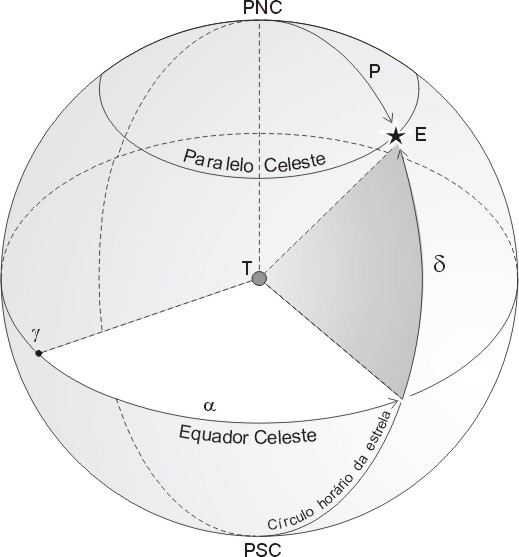
\includegraphics[width=0.58\linewidth]{figures/coords.png}
  \legend{Fonte: Núcleo Olímpico de Incentivo ao Conhecimento (NOIC). Disponível em: \url{https://noic.com.br/coordenadas-celestes}}
\end{figure}

Diversos sistemas de coordenadas são usados na astronomia, como o azimutal, o eclíptico e o equatorial. Esse último é amplamente usado na astronomia e o padrão em levantamentos astronômicos digitais (Seção \ref{sec:surveys}) sendo adotado como padrão nesse trabalho. Por isso, entender seus principais conceitos é fundamental para interpretar parte das figuras desse trabalho.

A Fig. \ref{fig:sistema-equatorial} mostra o sistema equatorial, composto pelas coordenadas de ascensão reta ($\alpha$ ou RA) e declinação ($\delta$ ou Dec). A ascensão reta é análoga à longitude e é medida em horas, minutos e segundos, ao longo do equador celeste, a partir do ponto vernal ($\gamma$), que é o ponto onde o Sol cruza o equador celeste na direção do hemisfério celestial norte durante o equinócio de março. A declinação, semelhante à latitude, é medida em graus acima ou abaixo do equador celeste, variando de $+90^{\circ}$ no polo celeste norte a $-90^{\circ}$ no polo celeste sul. O ponto $E$ na Fig. \ref{fig:sistema-equatorial}, marcado com uma estrela, representa um objeto celeste (ou astro) e pode ser definido pelo par de coordenadas $E = (\alpha, \delta)$.

Esse sistema de coordenadas é fundamental para a localização de objetos no céu e baseia-se no conceito da esfera celeste. A esfera celeste é uma representação imaginária do céu, uma superfície esférica de grande raio centrada na Terra (representada como o ponto T na Fig. \ref{fig:sistema-equatorial}), sobre a qual todos os objetos astronômicos parecem estar fixados. Essa concepção é útil porque facilita a definição de coordenadas angulares para descrever a posição de objetos no céu, similar ao sistema de latitude e longitude empregado na superfície terrestre. A esfera celeste é dividida por planos de referência como o equador celeste, que é a projeção do equador terrestre, e o eixo de rotação da Terra, que define os polos celestes norte (PNC) e sul (PSC).

A utilização da esfera celeste e das coordenadas equatoriais tem implicações significativas para as estruturas de dados empregadas em grandes catálogos astronômicos. Na próxima subseção, será discutido como explorar o conceito da esfera celeste para definir uma técnica eficiente de armazenamento e busca de objetos astronômicos.

% Dado o gigantesco volume de dados gerados por levantamentos astronômicos, é necessário desenvolver métodos eficientes para armazenar, processar e recuperar informações de forma precisa e rápida. Estruturas de dados específicas, como árvores de espaço de varredura (sky partitioning trees), k-d trees \cite{kdtree} e algoritmos baseados em hierarquias de pixels, como o sistema HEALPix \cite{healpix} e HIPS \cite{hips}, são amplamente utilizadas para indexar as posições dos objetos na esfera celeste. Essas estruturas permitem a divisão da esfera celeste em regiões menores e hierarquicamente organizadas, facilitando buscas eficientes e operações de vizinhança, que são essenciais em tarefas como a identificação de aglomerados de galáxias ou a execução de cruzamentos de dados entre diferentes levantamentos. Esse assunto será abordado com mais detalhes na próxima subseção.

% A representação esférica e as coordenadas angulares também impactam a precisão e a complexidade computacional dos algoritmos utilizados. Transformações de coordenadas, cálculos de distância angular e correções devido a efeitos astronômicos, como a aberração e a refração, devem ser tratados adequadamente para garantir a precisão dos dados astronômicos. Assim, a gestão de grandes catálogos astronômicos exige não apenas estratégias de armazenamento eficiente, mas também métodos robustos para garantir que as consultas e análises mantenham a precisão necessária para os estudos científicos que dependem desses dados.





% \subsection{Tesselação da Esfera Celeste}
% \label{sec:tesselacao}





\subsection{Levantamentos Astronômicos}
\label{sec:surveys}
Um levantamento astronômico consiste em uma pesquisa sistemática de grandes áreas do céu com o intuito de coletar dados sobre objetos e fenômenos celestes \cite[p. 40-42]{extragalactic-astronomy-book}. Estes levantamentos abrangem observações em diferentes faixas do espectro eletromagnético e buscam identificar e catalogar astros como estrelas, galáxias, aglomerados e nebulosas, fornecendo uma base de dados ampla e acessível para estudos detalhados \cite{astronomical-survey}. A finalidade dos levantamentos é construir um mapa celeste que permita compreender a distribuição e as propriedades dos corpos celestes em diversas escalas, auxiliando na análise estatística de populações estelares e galácticas e na identificação de estruturas de larga escala, como filamentos e vazios cósmicos \cite{bahcall1995,baleisis1998,jarrett2004}.

O grande volume de dados gerado por esses levantamentos astronômicos representa um desafio significativo. Os avanços em tecnologia de sensoriamento e armazenamento permitiram que telescópios modernos capturassem bilhões de objetos celestes em detalhes, gerando petabytes de dados que precisam ser processados, organizados e armazenados \cite{szalay2000,graefe1993}. Este volume de dados impõe desafios em termos de infraestrutura de armazenamento, processamento e análise, além de exigir métodos eficientes de organização e recuperação de informações. Para enfrentar esses desafios, foram desenvolvidos os chamados observatórios virtuais \cite{ivoa}, que integram e centralizam os dados provenientes de diversos levantamentos. Estes observatórios permitem o acesso distribuído aos dados e promovem a interoperabilidade entre diferentes conjuntos de dados, facilitando a análise conjunta de observações realizadas em diferentes regiões do espectro e por distintos instrumentos \cite{sciserver}.

A existência de múltiplos levantamentos astronômicos fotométricos se justifica pela necessidade de observar o universo em diferentes comprimentos de onda, uma vez que cada faixa do espectro revela características específicas dos objetos astronômicos. Por exemplo, a radiação ultravioleta é útil para identificar regiões de formação estelar intensa, enquanto o infravermelho é empregado na observação de regiões obscurecidas por poeira interestelar \cite[p. 28-31]{extragalactic-astronomy-book}. Assim, levantamentos em faixas distintas do espectro eletromagnético fornecem dados complementares que permitem uma visão mais completa dos processos físicos no cosmos. A variabilidade na profundidade (capacidade de observar objetos mais distantes e fracos) e na resolução espacial também diversifica os objetivos dos levantamentos. Nas próximas subseções, serão apresentadas breves descrições dos levantamentos utilizados no desenvolvimento deste projeto.


\subsubsection{Sloan Digital Sky Survey}
\label{sec:sdss}

\begin{figure}[!ht]
  \caption{Área de cobertura do levantamento SDSS}
  \label{fig:coverage-sdss}
  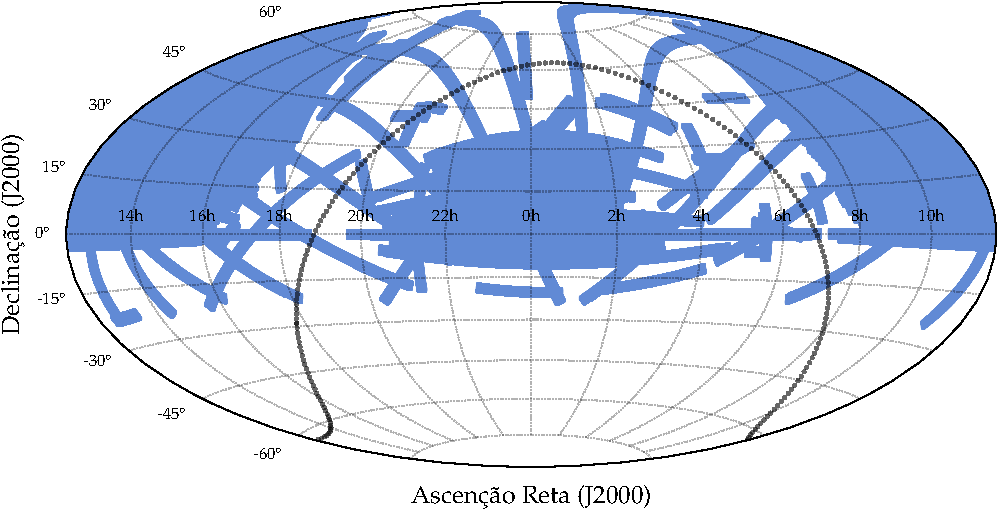
\includegraphics[width=\linewidth]{notebooks/plots/sdss_footprint.pdf}
  \legend{Fonte: autoria própria}
\end{figure}

O Sloan Digital Sky Survey\footnote{\url{https://sdss.org}} (SDSS; \citealp{sdss}) é um dos levantamentos astronômicos mais influentes e abrangentes, sendo pioneiro no uso de técnicas digitais para mapear o céu noturno. Iniciado em 2000, o SDSS empregou um telescópio dedicado de 2,5 metros \cite{sdss-telescope} equipado com uma poderosa câmera de dispositivo de carga acoplada (CCD;  \citealp{sdss-camera}) para mapear o céu do norte com detalhes sem precedentes, cobrindo uma área de cerca de 14.000 graus quadrados, principalmente no hemisfério celestial norte. A Fig. \ref{fig:coverage-sdss} mostra a área de cobertuda da décima oitava liberação de dados (DR18; \citealp{sdss-dr18}). Ao longo de suas diferentes fases, o levantamento produziu dados detalhados de milhões de estrelas, galáxias e quasares, contribuindo significativamente para o avanço de áreas como cosmologia, formação de galáxias e estrutura de larga escala do universo.

O SDSS foi um dos primeiros levantamentos a realizar observações em múltiplas bandas fotométricas, abrangendo cinco faixas do espectro eletromagnético: u, g, r, i e z \cite{sdss-filters}, com comprimentos de onda centrados em 3543 $\si{\angstrom}$, 4770 $\si{\angstrom}$, 6231 $\si{\angstrom}$, 7625 $\si{\angstrom}$ e 9134 $\si{\angstrom}$, respectivamente. Essas bandas cobrem desde o ultravioleta próximo até o infravermelho próximo, permitindo uma caracterização abrangente das propriedades físicas e químicas dos objetos observados. Esse mapeamento multiespectral fornece dados que possibilitam a estimativa de parâmetros astrofísicos, como temperatura e metalicidade, e facilita a classificação e estudo da evolução dos objetos celestes \cite{sdss-photo}.

O pioneirismo do SDSS como levantamento astronômico digital se destaca pela implementação de uma infraestrutura de dados digital chamada SkyServer\footnote{\url{https://skyserver.sdss.org}} \cite{skyserver} e de técnicas automatizadas para a aquisição e processamento das imagens \cite{sdss-photo} e dos espectros \cite{sdss-spec}. Os dados obtidos pelo SDSS foram disponibilizados ao público por meio de lançamentos periódicos, estabelecendo um novo padrão de acessibilidade e transparência na astronomia observacional. Esse levantamento digital não apenas tornou-se uma referência na organização e disseminação de dados, mas também promoveu o desenvolvimento de observatórios virtuais e inspirou a criação de novos levantamentos digitais em diferentes faixas espectrais, solidificando a transição para a era da astronomia baseada em big data \cite{sciserver}.





\subsubsection{Southern Photometric Local Universe Survey}
\label{sec:splus}

\begin{figure}[!ht]
  \caption{Área de cobertura do levantamento S-PLUS}
  \label{fig:coverage-splus}
  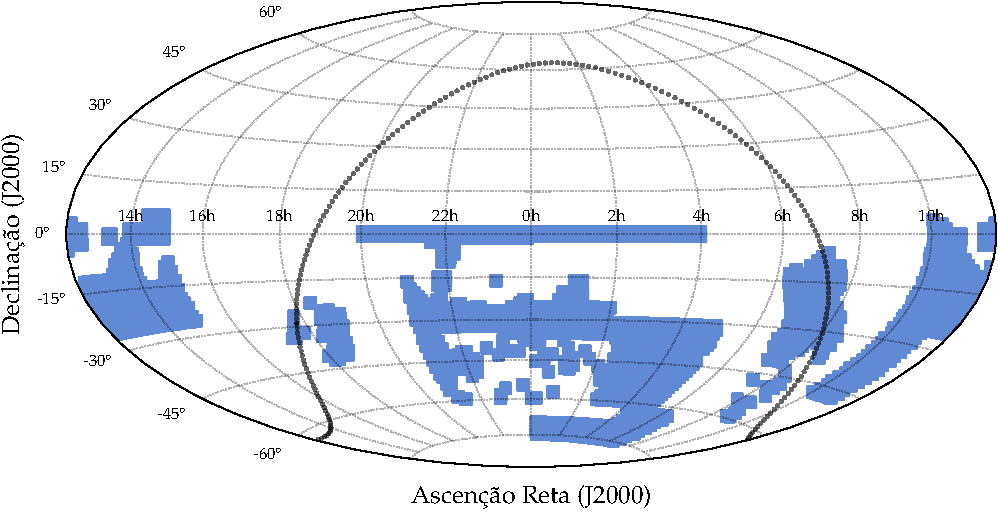
\includegraphics[width=\linewidth]{notebooks/plots/splus_footprint.pdf}
  \legend{Fonte: autoria própria}
\end{figure}

Em contraste com o SDSS, o levantamento astronômico brasileiro Southern Photometric Local Universe Survey\footnote{\url{https://splus.iag.usp.br}} (S-PLUS; \citealp{splus}) é um mapeamento do hemisfério celestial sul utilizando uma abordagem multibanda altamente detalhada. O S-PLUS utiliza o telescópio T80-Sul, localizado no Observatório de Cerro Tololo, no Chile, para observar uma área de aproximadamente 8.000 graus quadrados, como mostra a Fig. \ref{fig:coverage-splus}. Este levantamento cobre, portanto, uma ampla região do céu meridional, permitindo um estudo profundo de diversos objetos celestes, incluindo estrelas, galáxias e aglomerados de galáxias.

Um dos principais diferenciais do S-PLUS é a sua cobertura em doze bandas fotométricas, que incluem cinco bandas similares às do levantamento SDSS (u, g, r, i, z) e sete bandas estreitas (J0378, J0395, J0410, J0430, J0515, J0660, J0861) com comprimentos de onda variando entre 3780 $\si{\angstrom}$ e 8610 $\si{\angstrom}$. Essa configuração de bandas permite uma análise espectral rica, capturando detalhes como a presença de linhas de emissão e absorção específicas, que são cruciais para a determinação precisa de parâmetros físicos e químicos dos objetos observados. Por exemplo, as bandas estreitas foram escolhidas para registrar características específicas como o traço do cálcio, magnésio e oxigênio, o que facilita a análise da composição estelar e a identificação de processos de formação estelar. Como levantamento astronômico digital, o S-PLUS disponibiliza seus dados para a comunidade científica em um formato acessível e padronizado através da plataforma S-PLUS Cloud (\url{https://splus.cloud}), promovendo a interoperabilidade com outros levantamentos e incentivando o desenvolvimento de estudos complexos em astronomia observacional e cosmologia.




\subsubsection{Legacy Surveys}
\label{sec:legacy}
\begin{figure}[!ht]
  \caption{Área de cobertura do levantamento DESI Legacy Survey}
  \label{fig:coverage-legacy}
  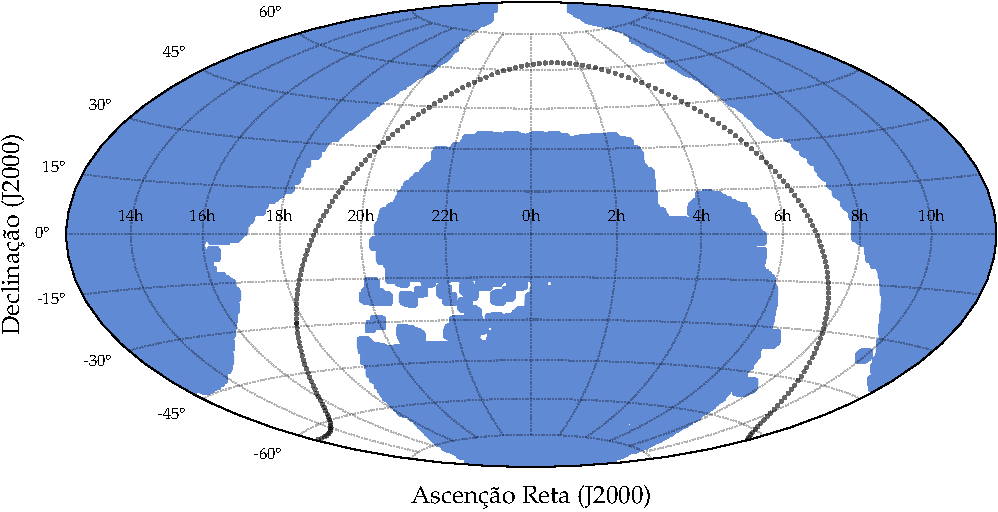
\includegraphics[width=\linewidth]{notebooks/plots/legacy_footprint.pdf}
  \legend{Fonte: autoria própria}
\end{figure}


Os Legacy Surveys\footnote{\url{https://legacysurvey.org}} \cite{legacy} consistem em três projetos individuais e complementares: o Dark Energy Camera Legacy Survey (DECaLS), o Beijing-Arizona Sky Survey (BASS) e o Mayall z-band Legacy Survey (MzLS). Juntos, formam um dos maiores projetos de mapeamento digital do céu, projetado para fornecer uma base fotométrica abrangente para o projeto Dark Energy Spectroscopic Instrument (DESI). O Legacy Survey cobre aproximadamente 14.000 graus quadrados do céu. Esse levantamento oferece uma cobertura profunda e em múltiplas bandas fotométricas, incluindo as bandas $g$, $r$ e $z$, com comprimentos de onda centrados em aproximadamente 4750 Å, 6300 Å e 9200 Å, respectivamente. Essas bandas, juntamente com sua grande profundidade, permitem a detecção de objetos mais fracos e distantes, possibilitando estudos detalhados da distribuição de galáxias e outras estruturas em grandes escalas.

A profundidade dos Legacy Surveys é um dos fatores que o diferencia de outros levantamentos, como o SDSS e o S-PLUS. Com exposições projetadas para alcançar uma profundidade mais elevada, os Legacy Surveys são capazes de detectar objetos com brilho mais tênue, o que é fundamental para o mapeamento detalhado da estrutura de larga escala do universo.
%Este aspecto é essencial para o projeto DESI, que utiliza os dados do Legacy Survey para selecionar alvos para espectroscopia, a fim de estudar a energia escura e a expansão cósmica. 
Em comparação, o SDSS foi um dos primeiros levantamentos digitais a mapear o céu com precisão em cinco bandas, mas com uma profundidade moderada, voltada para observações mais próximas. Já o S-PLUS, com suas doze bandas, fornece uma caracterização espectral mais detalhada de cada objeto, mas com um foco em uma área específica do céu no hemisfério celestial sul e uma profundidade relativamente menor em comparação com os Legacy Surveys.

Assim, enquanto o SDSS estabeleceu o padrão para levantamentos digitais de grande escala, e o S-PLUS trouxe um detalhamento espectral fino com bandas estreitas, os Legacy Surveys combinam uma ampla cobertura com alta profundidade, posicionando-se como uma base essencial para o estudo da cosmologia e da estrutura de larga escala do universo. A integração desses levantamentos complementares permite uma análise mais completa do céu, tanto em termos de área quanto de profundidade e detalhamento espectral, promovendo avanços em diversas áreas da astronomia e da astrofísica.





\subsection{Padrões e Protocolos na Astronomia}
\label{sec:protocolos}

Os padrões e protocolos são fundamentais para a pesquisa em astronomia, principalmente devido ao crescente volume e à diversidade dos dados astronômicos disponíveis. Como abordado na seção anterior, cada levantamento astronômico tem um propósito específico, observando fenômenos físicos distintos (a partir de escolhas tomadas na contrução do equipamento, como os comprimentos de onda observados, a quantidade de filtros e a resolução da câmera) em diferentes regiões do céu. Nesse sentido, a padronização é essencial para garantir que  fontes de dados distintas sejam acessíveis e compatíveis entre si. Ao adotar padrões, torna-se possível integrar informações de diferentes observatórios e levantamentos, facilitando a reutilização de dados e promovendo estudos comparativos em larga escala. Isso cria um ecossistema em que dados de múltiplos projetos podem ser analisados de maneira conjunta, ampliando a possibilidade de descobertas científicas que dependem da integração de informações heterogêneas.

Os protocolos da International Virtual Observatory Alliance\footnote{\url{https://ivoa.net}} (IVOA; \citealp{ivoa}) desempenham um papel crucial na astronomia, viabilizando a interoperabilidade, o acesso e a utilização de dados astronômicos provenientes de diferentes observatórios e levantamentos. Criados para unificar e padronizar o compartilhamento e a manipulação de dados, esses protocolos compõem uma estrutura abrangente e organizada que facilita o intercâmbio de informações em um ambiente colaborativo global. Com a crescente quantidade e diversidade dos dados astronômicos, o IVOA estabelece normas que garantem que informações oriundas de várias fontes possam ser integradas e acessadas de maneira consistente, independente do formato ou origem, fomentando avanços na pesquisa astronômica.

O conjunto de protocolos IVOA é estruturado em diversas camadas, que funcionam de forma integrada para compor o ambiente de serviço do Observatório Virtual (VO; \citealp{voarch}). A \emph{Camada de Protocolos de Acesso a Dados} é uma das principais e inclui o Data Access Layer Interface (DALI; \citealp{dali}), que define os princípios gerais de interação com serviços de dados, o Table Access Protocol (TAP; \citealp{tap}) para acesso a tabelas, e os protocolos especializados como o Simple Cone Search (SCS; \citealp{scs}), o Simple Spectral Access Protocol (SSAP; \citealp{ssa}) e o Simple Image Access Protocol (SIAP; \citealp{siap}), que facilitam o acesso a catálogos, espectros e imagens, respectivamente. Essas ferramentas possibilitam que os usuários recuperem informações específicas em diferentes bases de dados astronômicas. Por outro lado, a \emph{Camada de Serviços} gerencia a integração de serviços, com o uso de ferramentas como o Universal Worker Service (UWS; \citealp{uws}) para coordenar tarefas assíncronas em servidores de dados.

Além dos protocolos de acesso, a \emph{Camada de Formatos} define como os dados devem ser representados e trocados. Os formatos VOTable \cite{votable}, usado para tabelas de dados, e FITS \cite{fits}, adotado tanto para imagens e tabelas, garantem que os dados sejam armazenados de forma padronizada, permitindo sua compatibilidade e compreensão entre diferentes sistemas. Já os \emph{Modelos de Dados} \cite{vomodel} especificam a estrutura e o significado dos dados, fornecendo uma semântica comum para que diferentes sistemas interpretem corretamente o conteúdo dos catálogos e tabelas. Por exemplo, os modelos incluem descrições de propriedades como fluxos, coordenadas e características espectrais, facilitando comparações e agregações de dados de diferentes fontes.

A \emph{Camada de Protocolos Semânticos} inclui padrões como Unified Content Descriptors (UCD; \citealp{ucd}), que proporciona uma nomenclatura padronizada para descrever o conteúdo dos dados, e o VOUnit \cite{vounit}, que define unidades de medida de forma consistente. Esses protocolos semânticos são essenciais para assegurar que os dados sejam interpretados corretamente por pesquisadores e softwares, evitando ambiguidades e promovendo uma compreensão clara dos conjuntos de dados. Por outro lado, o uso de linguagens de consulta, como a Astronomical Data Query Language (ADQL; \citealp{adql}), oferece uma sintaxe padronizada para a realização de consultas avançadas em bancos de dados astronômicos, permitindo filtragens e extrações complexas diretamente nos repositórios de dados do VO.

A interação entre essas camadas cria um ambiente de serviço VO em que cada componente desempenha um papel específico para garantir que os dados possam ser acessados, analisados e interpretados de forma integrada. Essa integração e padronização é fundamental para a operação automatizada de um sistema inteligente para descoberta em astronomia. %Por exemplo, um pesquisador pode usar ADQL para definir uma consulta complexa que é executada por meio do TAP, recuperando tabelas em formato VOTable com descrições de conteúdo padronizadas por UCD. Essa infraestrutura permite que dados de diferentes observatórios e levantamentos, armazenados de forma distribuída, sejam utilizados de maneira conjunta, promovendo uma pesquisa colaborativa e eficiente.


% \subsubsection{Camada de Dados}


% \begin{quadro}
%   \caption{Broca}
%   \begin{lstlisting}[language=xml,caption={Broca}]
% <?xml version="1.0" encoding="UTF-8"?>
% <VOTABLE version="1.4">
%   <RESOURCE name="myFavouriteGalaxies">
%     <COOSYS ID="sys" equinox="J2000" epoch="J2000" />
%     <TABLE name="results">
%       <DESCRIPTION>Velocities estimations</DESCRIPTION>
%       <PARAM name="Telescope" ucd="phys.size"  
%              datatype="float" unit="m" value="3.6"/>
%       <FIELD name="RA" ucd="pos.eq.ra" datatype="float"
%              width="6" precision="2" unit="deg" ref="sys"/>
%       <FIELD name="Dec" ucd="pos.eq.dec" datatype="float"
%              width="6" precision="2" unit="deg" ref="sys"/>
%       <FIELD name="vel" ucd="spect.dopplerVeloc" 
%              width="5" datatype="int" unit="km/s"/>
%       <FIELD name="e_vel" ucd="stat.error;spect.dopplerVeloc" 
%              width="3" datatype="int" unit="km/s">
%         <DESCRIPTION>Distance of Galaxy</DESCRIPTION>
%       </FIELD>
%       <DATA>
%         <TABLEDATA>
%         <TR>
%           <TD>010.68</TD><TD>+41.27</TD><TD>-297</TD><TD>5</TD>
%         </TR>
%         <TR>
%           <TD>287.43</TD><TD>-63.85</TD><TD>839</TD><TD>6</TD>
%         </TR>
%         </TABLEDATA>
%       </DATA>
%     </TABLE>
%   </RESOURCE>
% </VOTABLE>
% \end{lstlisting}
% \end{quadro}



% \subsubsection{Camada de Acesso aos Dados}


% \subsection{Exploração de Catálogos Astronômicos}
% \subsubsection{Busca em Cone}

% \subsubsection{Correlação}


\subsection{Morfologia}
\label{sec:morfologia}

Na astronomia, morfologia refere-se ao estudo das formas e das estruturas observáveis dos objetos celestes, como galáxias, nebulosas, estrelas e aglomerados estelares \cite{buta2011galaxy}. A análise morfológica busca descrever e categorizar as características visuais desses objetos, identificando padrões estruturais que possam fornecer percepções sobre seus processos de formação e evolução \cite{steinmetz2002galaxy}. Em particular, as galáxias são frequentemente classificadas com base em sua morfologia. Essas classificações refletem características como a distribuição de estrelas, a presença de braços espirais e a concentração de massa no núcleo, o que está diretamente associado à dinâmica interna e ao histórico evolutivo de cada galáxia \cite{van1998galaxy}.

\subsubsection{Raio Efetivo}
\label{sec:raio-efetivo}

O raio efetivo de uma galáxia é uma medida fundamental em astronomia que caracteriza a distribuição espacial de sua luminosidade. Em termos práticos, o raio efetivo é definido como a distância do centro da galáxia até o ponto onde metade da luz total emitida galáxia está concentrada. Essa métrica é amplamente utilizada para descrever a extensão aparente das galáxias e fornece informações valiosas sobre sua estrutura interna e dinâmica.

O cálculo do raio efetivo depende da análise da distribuição de brilho da galáxia, sendo comumente obtido por meio de perfis de brilho de superfície que representam a intensidade luminosa em função da distância ao centro da galáxia. Para galáxias elípticas, esses perfis de brilho são tipicamente modelados por uma distribuição de Sérsic, que se ajusta bem à sua estrutura concentrada. Já para galáxias espirais, a distribuição de brilho tende a ser mais complexa, com um núcleo brilhante e uma extensão de braços espirais, o que pode exigir ajustes mais detalhados para determinar o raio efetivo.

\subsubsection{Elipticidade}
\label{sec:elipticidade}

A elipticidade complexa é uma métrica amplamente utilizada em estudos de lentes gravitacionais, onde se faz necessária a quantificação precisa da distorção observada nas imagens de objetos distantes devido à ação gravitacional de um objeto massivo interveniente, como uma galáxia ou um aglomerado de galáxias. Essa métrica é essencial para descrever a forma das imagens distorcidas, permitindo a análise da distribuição de massa do objeto que atua como lente. Especificamente, a elipticidade complexa captura a deformação das fontes de luz distantes sob a forma de uma componente elíptica, expressando tanto a intensidade da distorção (ou seja, o alongamento da imagem) quanto a sua orientação no plano do céu.

A métrica de elipticidade complexa é particularmente útil na modelagem e análise de lentes fracas, em que as distorções são sutis e a forma das galáxias de fundo serve como uma sonda estatística para inferir a presença de matéria escura e a estrutura da lente gravitacional. Essa métrica desempenha um papel crucial para estudos que investigam a distribuição de matéria escura e a formação de grandes estruturas no universo. Ao quantificar a distorção induzida por lentes gravitacionais, os astrônomos podem mapear a distribuição de massa em escalas cósmicas, incluindo matéria que não emite luz visível, como a matéria escura. Em estudos de lenteamento fraco, onde os efeitos de distorção são mínimos e requerem uma análise estatística sobre grandes populações de galáxias, a elipticidade complexa oferece uma forma consistente e precisa de capturar e interpretar essas pequenas distorções.


\subsubsection{Brilho e Magnitude}
\label{sec:magnitude}

O brilho e a magnitude são conceitos fundamentais para quantificar a intensidade de luz emitida ou refletida por objetos celestes, sendo essenciais para a caracterização de estrelas, galáxias e outros corpos celestes. O brilho refere-se à quantidade total de energia luminosa recebida por unidade de área em um detector, como um telescópio. É uma medida física direta da intensidade de luz e varia inversamente com o quadrado da distância do objeto, sendo comumente expresso em termos de fluxo, que é a quantidade de luz recebida por unidade de área por unidade de tempo. A medição do brilho permite aos astrônomos determinar características intrínsecas dos objetos, como temperatura e tamanho, e é um dos parâmetros centrais para estudar a evolução estelar e a estrutura galáctica.

A magnitude, por outro lado, é uma medida que descreve o brilho percebido dos objetos astronômicos em escala logarítmica, introduzida para lidar com a vasta gama de intensidades luminosas observadas no céu. A escala de magnitude é inversa, de forma que objetos mais brilhantes têm magnitudes menores, enquanto objetos mais fracos têm magnitudes maiores. A magnitude aparente quantifica o brilho de um objeto visto da Terra, enquanto a magnitude absoluta define o brilho que o objeto teria se estivesse a uma distância padrão de 10 parsecs. Essa distinção permite que astrônomos comparem o brilho intrínseco de diferentes objetos, independentemente de sua distância da Terra.


\subsubsection{Classificação Morfológica}
\label{sec:classificao}

A classificação morfológica é um sistema de categorização utilizado em astronomia para descrever e agrupar galáxias com base em suas características estruturais e visuais. Esse processo é fundamentado em características observáveis, como a forma, a distribuição de luminosidade, a presença de braços espirais ou um núcleo central proeminente \cite{steinmetz2002galaxy}. A classificação morfológica permite organizar galáxias em grupos que compartilham propriedades físicas e evolutivas semelhantes, facilitando o estudo de sua formação, dinâmica e história evolutiva. Esse sistema é especialmente valioso na astronomia observacional, onde padrões morfológicos podem ser correlacionados com fenômenos físicos específicos, como fusões e interações gravitacionais entre galáxias \cite{van1998galaxy}.

Historicamente, o primeiro sistema de classificação morfológica foi desenvolvido por \citeonline{hubble1926}, que introduziu o ``diagrama de diapasão'' para agrupar galáxias em três principais categorias: elípticas, espirais e irregulares. Esse esquema básico de Hubble, também chamado de sequência de Hubble, organizava as galáxias de acordo com sua forma e estrutura, identificando uma possível progressão evolutiva entre os tipos. As galáxias elípticas, por exemplo, são caracterizadas por uma distribuição suave e arredondada de luz e pouca formação estelar, enquanto as espirais possuem braços bem definidos e núcleos brilhantes, indicando regiões de intensa formação de estrelas. As galáxias irregulares, por sua vez, apresentam formas menos definidas e são frequentemente associadas a perturbações gravitacionais.

A importância da classificação morfológica na astronomia reside na sua capacidade de revelar padrões fundamentais sobre a evolução das galáxias e do universo como um todo. A morfologia galáctica não apenas reflete o estado atual de uma galáxia, mas também oferece pistas sobre sua história dinâmica, como colisões passadas, interações com outras galáxias e a presença de matéria escura. Por meio da classificação morfológica, os astrônomos podem investigar como as diferentes populações de galáxias variam ao longo do tempo cósmico, relacionando suas características estruturais com fatores como a densidade do ambiente e a quantidade de gás disponível para a formação estelar. Assim, a classificação morfológica se consolida como um método essencial para compreender a formação e evolução das galáxias, contribuindo para um entendimento mais profundo sobre a estrutura e a dinâmica do universo.



\section{Ciência Cidadã}
\label{sec:cs}
A ciência cidadã é um campo interdisciplinar emergente que envolve a participação ativa do público geral em tarefas de pesquisas científicas com finalidade de produzir novos conhecimentos para a ciência e para a sociedade \cite{scs-1}, especialmente na coleta, categorização, transcrição e análise de dados científicos \cite{silvertown2009,bonney2014}. Este modelo de pesquisa tem ganhado relevância em diversos campos da ciência, principalmente devido ao aumento do acesso a tecnologias digitais e à internet, que facilitam a comunicação e a organização entre cidadãos e cientistas \cite{scs-4}.
%No decorrer dessa seção, será feito um breve levantamento do uso da ciência cidadã em diferentes áreas do conhecimento (Seção \ref{sec:cs-areas}), bem como na astronomia (Seção \ref{sec:cs-astro}), e uma perspectiva sobre a qualidade dos dados gerados (Seção \ref{sec:cs-data-quality}).

Na astronomia, o GalaxyZoo\footnote{\url{https://galaxyzoo.org}} \cite{gz} é um projeto de ciência cidadã lançado em 2007, cujo objetivo é classificar morfologicamente galáxias utilizando imagens obtidas por grandes levantamentos astronômicos, como o Sloan Digital Sky Survey (SDSS). Os participantes, voluntários de diferentes formações e níveis de conhecimento científico, analisam imagens de galáxias e fornecem informações sobre suas características, como forma espiral, elíptica ou irregular, e a presença de estruturas específicas, como barras centrais. Essa colaboração massiva permitiu a classificação de milhões de galáxias em um curto período, superando em eficiência o que seria possível com equipes científicas tradicionais.

O impacto científico do GalaxyZoo é expressivo. Além de fornecer uma base de dados robusta e de alta qualidade para a pesquisa astronômica, o projeto gerou avanços no entendimento da formação e evolução de galáxias, incluindo a relação entre morfologia e ambiente. Os resultados têm sido utilizados para treinar modelos de aprendizado de máquina, permitindo a automação de tarefas de classificação em levantamentos futuros. O sucesso do GalaxyZoo também inspirou o desenvolvimento de outras plataformas de ciência cidadã, consolidando seu papel como ferramenta metodológica na pesquisa científica.

Para os voluntários, o GalaxyZoo oferece uma oportunidade de engajamento direto com a ciência, promovendo aprendizado e um senso de contribuição para descobertas científicas relevantes. Muitos participantes relatam um aumento na compreensão de conceitos astronômicos e motivação para explorar outras áreas da ciência. Além disso, a plataforma fomenta uma comunidade global de entusiastas que colaboram ativamente, monstando como iniciativas bem estruturadas podem democratizar o acesso e a participação no progresso científico.



% \subsection{Áreas de Atuação da Ciência Cidadã}
% \label{sec:cs-areas}
% \lipsum[4]


% \subsection{Ciência Cidadã na Astronomia}
% \label{sec:cs-astro}
% \lipsum[4]


% \subsection{Qualidade dos Dados}
% \label{sec:cs-data-quality}
% \lipsum[4]







\section{Aprendizagem Profunda}
\label{sec:dl}

A aprendizagem profunda, ou deep learning, é uma subárea da inteligência artificial (IA) que envolve o uso de redes neurais artificiais com múltiplas camadas para modelar e processar dados complexos. Inspirada inicialmente na estrutura e no funcionamento do cérebro humano, essa abordagem visa reproduzir, em um ambiente computacional, a capacidade do cérebro de identificar padrões e inferir informações a partir de grandes volumes de dados. O termo ``profunda'' refere-se ao uso de várias camadas ocultas na rede neural, que permite que modelos de aprendizagem profunda extraiam hierarquias de características complexas, aumentando a precisão e a capacidade do modelo em resolver problemas como reconhecimento de fala, visão computacional e processamento de linguagem natural.

% Historicamente, a aprendizagem profunda teve suas raízes no desenvolvimento das redes neurais artificiais nos anos 1940 e 1950, com o modelo de perceptron proposto por Frank Rosenblatt e os trabalhos teóricos de Warren McCulloch e Walter Pitts, que estabeleceram o conceito de neurônio artificial. Nos anos 1980, o desenvolvimento do algoritmo de retropropagação, por Geoffrey Hinton e outros pesquisadores, possibilitou o ajuste de redes neurais multicamadas, mas a limitação computacional da época impediu sua adoção generalizada. Somente na década de 2000, com o aumento da capacidade computacional, a disponibilidade de grandes conjuntos de dados e o aprimoramento de técnicas como redes convolucionais (CNNs) e redes recorrentes (RNNs), a aprendizagem profunda ressurgiu e demonstrou um desempenho superior em várias tarefas de IA.

% O impacto da aprendizagem profunda em pesquisas científicas baseadas em dados é imensurável, transformando a maneira como diferentes disciplinas lidam com grandes volumes de dados. Em astronomia, por exemplo, algoritmos de aprendizagem profunda são amplamente aplicados na classificação de galáxias, detecção de exoplanetas e identificação de anomalias em dados astronômicos, onde o volume de informações é tão grande que métodos tradicionais de análise se tornam inviáveis. Na área de saúde, redes neurais profundas auxiliam no diagnóstico de doenças e na análise de imagens médicas, permitindo a identificação precoce de condições como câncer e doenças cardiovasculares com um nível de precisão cada vez maior. A aprendizagem profunda também desempenha um papel crucial no avanço da bioinformática, modelando interações entre proteínas e genomas em um nível detalhado e acelerando a descoberta de novos medicamentos.

% A capacidade da aprendizagem profunda de extrair e organizar informações relevantes a partir de dados não estruturados é um fator chave para sua adoção em pesquisas científicas, onde muitos dos dados disponíveis apresentam características complexas e pouco lineares. Modelos profundos conseguem identificar padrões de maneira hierárquica, onde as primeiras camadas da rede extraem características mais gerais, como bordas e formas, enquanto camadas mais profundas identificam aspectos mais específicos e complexos. Esse comportamento hierárquico, aliado à capacidade de generalização desses modelos, permite que a aprendizagem profunda vá além das abordagens tradicionais de análise estatística, trazendo uma nova perspectiva para a análise de dados e impulsionando descobertas científicas.

% Além disso, a aprendizagem profunda continua a evoluir, com o desenvolvimento de técnicas como redes generativas adversariais (GANs), redes neurais transformadoras e modelos de transferência de aprendizagem. Essas inovações têm potencial para lidar com problemas ainda mais complexos e para serem aplicadas em cenários de dados escassos ou em tarefas de aprendizado contínuo. Em resumo, a aprendizagem profunda representa uma revolução na capacidade de processamento e análise de dados, impactando amplamente o avanço do conhecimento científico e possibilitando que diferentes campos explorem de maneira inédita as grandes quantidades de dados disponíveis.

\subsection{Redes Neurais}
\label{sec:ann}

As redes neurais artificiais são modelos computacionais inspirados no funcionamento do cérebro humano, constituídos por unidades denominadas ``neurônios artificiais'' interligados em uma estrutura de camadas. Esses modelos buscam simular a capacidade do cérebro de reconhecer padrões, processar informações e realizar tarefas complexas de forma autônoma. A estrutura básica de uma rede neural é composta por uma camada de entrada, uma ou mais camadas ocultas e uma camada de saída. Cada camada possui neurônios conectados por pesos que são ajustados durante o processo de treinamento, permitindo que a rede aprenda a realizar tarefas específicas.

O desenvolvimento das redes neurais artificiais remonta aos anos 1940, com os trabalhos de \citeonline{neuronio}, que propuseram o primeiro modelo de neurônio artificial. Nos anos 1960, o perceptron, desenvolvido em \citeonline{perceptron}, trouxe um avanço significativo, sendo capaz de resolver problemas lineares simples. No entanto, o perceptron era limitado a problemas linearmente separáveis. Duas décadas depois, ocorreu um significativo avanço que permitiu que redes neurais resolvessem problemas não-lineares: a introdução do algoritmo de retropropagação de erro, proposto em \citeonline{backprop}, que possibilitou o treinamento de redes com múltiplas camadas ocultas, abrindo caminho para a evolução do campo.


\subsection{Aprendizado Profundo em Visão Computacional}
\label{sec:dl-cv}
A partir dos anos 2000, o aumento da capacidade computacional e o acesso a grandes volumes de dados catalisaram o desenvolvimento das redes neurais profundas, ou aprendizagem profunda. As redes neurais profundas (ou deep learning) são redes com múltiplas camadas ocultas, que permitem a extração de representações complexas e hierárquicas dos dados. Modelos profundos, como as redes neurais convolucionais (CNNs) e as redes neurais recorrentes (RNNs), provaram ser extremamente eficazes em tarefas de reconhecimento de imagem, processamento de linguagem natural e até mesmo na descoberta de novas partículas na física, evidenciando seu potencial em diversas áreas científicas.

Durante a última década, a aprendizagem profunda conquistou um notório sucesso em visão computacional devido sua capacidade de processamento de dados complexos, exercendo um impacto profundo nas pesquisas científicas, especialmente naquelas baseadas em grandes volumes de dados, como astronomia \cite{astro1, astro2}, medicina \cite{VGG16Ex03, InceptionResNetV2Ex03, InceptionResNetV2Ex02} e agronomia \cite{EfficientNetEx03, VGG16Ex02}. Isso se iniciou com as primeiras arquiteturas convolucionais profundas, como AlexNet \cite{alexnet-x} e VGG \cite{vgg16-x}, passando por Inception \cite{inception-x}, ResNet \cite{resnet-x} e EfficientNet \cite{efficientnet-x}, até chegar nos modelos baseados em transformadores \cite{transformers-x}, como Vision Transformer \cite{vit} e Swin Transformer \cite{swin}, além de arquiteturas híbridas como Multi-axis Vision Transformer \cite{maxvit} e Fast Vision Transformer \cite{fastvit}. Todos esses modelos dependem de um grande volume de dados para serem treinados, como ImageNet \cite{imagenet-x}, MS-COCO \cite{ms-coco} ou até maiores. Isso nos leva a entender que o avanço da capacidade preditiva dos modelos de visão computacional é, essencialmente, sustentado pelo aumento da complexidade do modelo e, consequentemente, por um grande conjunto de treinamento.

% O impacto da aprendizagem profunda em pesquisas científicas baseadas em dados é impulsionado pela capacidade das redes neurais de aprender representações complexas e identificar padrões intrínsecos nos dados. As camadas profundas dessas redes extraem características de baixo nível, como bordas e texturas, nas camadas iniciais, e informações de alto nível, como formas e estruturas complexas, nas camadas mais profundas. Essa capacidade de representação hierárquica permite que redes neurais profundas adaptem-se a uma vasta gama de problemas, oferecendo soluções inovadoras e ampliando as fronteiras do conhecimento em áreas científicas que exigem análises precisas e complexas.

% A evolução das redes neurais e a consolidação da aprendizagem profunda transformaram a forma como se realiza pesquisa científica atualmente, proporcionando ferramentas poderosas para a análise de dados e a descoberta de padrões. À medida que novas arquiteturas de redes, como redes generativas adversariais (GANs) e transformadores, continuam a ser desenvolvidas, espera-se que o impacto da aprendizagem profunda se expanda ainda mais, promovendo avanços em áreas como física de partículas, ciência dos materiais e previsão de fenômenos climáticos, onde a análise de dados é essencial para o desenvolvimento de novos conhecimentos.

\subsection{Recuperação de Imagens Baseado em Conteúdo}
\label{sec:cbir}

A recuperação de imagem baseada em conteúdo (CBIR) é uma tarefa de grande relevância na área de visão computacional, que consiste em buscar imagens em um banco de dados utilizando características visuais extraídas automaticamente, em vez de depender de metadados ou descrições textuais. O objetivo principal dessa abordagem é identificar imagens visualmente similares à consulta fornecida pelo usuário, considerando atributos como cor, textura, forma ou padrões visuais específicos.

Inicialmente, as técnicas de CBIR baseavam-se em métodos tradicionais de extração de características. Algoritmos como histogramas de cor, transformadas para análise de textura (como Gabor) e detectores de bordas (como Canny) eram amplamente utilizados. Essas abordagens geravam descritores manuais, que eram comparados utilizando métricas de similaridade, como distância euclidiana ou similaridade do cosseno. Apesar de funcionais, esses métodos eram limitados pela incapacidade de capturar características semânticas mais complexas, o que frequentemente resultava em baixa precisão em bancos de dados heterogêneos.

Com os avanços em aprendizado profundo, a utilização de redes neurais convolucionais (Convolutional Neural Networks, CNNs) transformou a abordagem de CBIR. As CNNs possuem a capacidade de aprender representações hierárquicas diretamente dos dados, extraindo características visuais de baixo nível (como bordas) e abstrações de alto nível (como formas e contextos). Essas representações visuais extraídas são codificadas em forma de vetores, também chamados de \emph{embeddings}. Por isso, modelos de aprendizado profundo tornaram-se ferramentas comuns para gerar tais representações visuais das imagens, que podem ser armazenadas e comparadas eficientemente. Essa abordagem não apenas melhora a precisão da recuperação, mas também permite lidar com variações de escala, rotação e iluminação das imagens.

As implementações mais avançadas de CBIR empregam técnicas como aprendizado de métrica e redes neurais siamêsas para otimizar diretamente a tarefa de similaridade visual. Além disso, combinações de embeddings extraídos de CNNs com informações adicionais, como metadados ou descrições textuais, têm sido exploradas para sistemas mais robustos e contextualmente relevantes. Em aplicações complexas, como astronomia ou medicina, onde os bancos de dados são massivos e as diferenças sutis entre imagens são críticas, essas técnicas modernas têm mostrado eficácia superior, tornando a CBIR uma ferramenta essencial para análise de dados e descoberta científica.

% \subsection{Visão Computacional}
% \label{sec:cv}

% \subsection{Recuperação de Imagens Baseada em Conteúdo}
% \label{sec:cbir}



\section{Sistemas de Informação}
\label{sec:sistemas-informacao}
\subsection{Bancos de Dados Relacionais}

Um banco de dados relacional \cite{relational-database,relational-database-2} é um sistema de armazenamento e organização de dados que utiliza o modelo relacional para estruturar as informações em tabelas, ou relações, permitindo um acesso eficiente e seguro aos dados armazenados. Nesse modelo, cada tabela é composta por linhas e colunas, onde as linhas representam registros (ou tuplas) e as colunas representam os atributos (ou campos) que descrevem as características de cada registro. Essa organização de dados possibilita o estabelecimento de relações entre as tabelas por meio de chaves primárias e chaves estrangeiras, facilitando a associação de informações de diferentes tabelas com base em valores comuns.

A principal característica do modelo relacional é a independência dos dados, que permite que as informações sejam manipuladas sem que o usuário precise conhecer detalhes do armazenamento físico. Os dados são acessados e manipulados por meio da Structured Query Language (SQL; \citealp{sequel}), uma linguagem de consulta declarativa que permite a execução de operações como inserção, atualização, exclusão e recuperação de dados.

A integridade e a consistência dos dados em um banco de dados relacional são asseguradas pelo uso de restrições e transações. As restrições, como as de chave primária, chave estrangeira e unicidade, garantem que os dados mantêm-se válidos de acordo com as regras estabelecidas para cada relação. As transações, por sua vez, permitem que múltiplas operações sejam executadas de forma atômica, garantindo que, em caso de falha, o banco de dados possa retornar a um estado consistente, preservando a integridade das informações.

Os bancos de dados relacionais são amplamente utilizados em diversas aplicações, desde sistemas de gestão empresarial até plataformas de e-commerce e redes sociais, devido à sua capacidade de organizar e manipular grandes volumes de dados de maneira eficaz. Entre os sistemas de gerenciamento de bancos de dados relacionais (SGBDs) mais populares estão o MySQL, PostgreSQL, Oracle e SQL Server, cada um oferecendo características e funcionalidades específicas para atender às necessidades de diferentes tipos de aplicações.


\subsubsection{API RESTful}
Uma Interface de Programação de Aplicação (API) Representational State Transfer (RESTful) são interfaces de comunicação amplamente utilizadas no desenvolvimento de sistemas de informação baseados em tecnologias web. Fundamentadas no protocolo HTTP, essas APIs seguem princípios arquiteturais que definem interações padronizadas e escaláveis entre sistemas, utilizando métodos como GET, POST, PUT e DELETE para realizar operações relacionadas a recursos. Os recursos são identificados por URLs e geralmente representados em formatos como JSON ou XML, o que facilita a interoperabilidade entre diferentes plataformas e linguagens de programação.

No contexto de um sistema de informação baseado em tecnologias web, as APIs RESTful desempenham um papel central ao possibilitar a comunicação entre o backend e o frontend, além de integrar serviços externos. Por exemplo, em um sistema de recuperação de imagens por similaridade visual, a API pode gerenciar solicitações de busca enviadas pelo usuário, consultar bancos de dados para encontrar imagens relevantes e retornar os resultados no formato apropriado. Sua estrutura modular e desacoplada permite que diferentes componentes do sistema evoluam de forma independente, garantindo flexibilidade para adaptações futuras.


\subsubsection{Aplicações Web Modernas}

Aplicações web modernas são sistemas dinâmicos e interativos projetados para fornecer experiências de usuário fluidas, muitas vezes comparáveis às de aplicações desktop. Essas aplicações aproveitam arquiteturas baseadas em tecnologias web avançadas, como APIs RESTful e frameworks de frontend, para oferecer funcionalidades ricas e responsivas. Diferentemente de aplicações web tradicionais, onde a interação frequentemente exige recarregamentos completos da página, as modernas utilizam técnicas como renderização dinâmica e atualizações assíncronas para otimizar a interação e reduzir a latência percebida pelo usuário.

Um dos pilares no desenvolvimento de aplicações web modernas é o uso de bibliotecas de frontend como React\footnote{\url{https://react.dev}}. O React facilita a construção de interfaces de usuário por meio de componentes reutilizáveis e uma abordagem declarativa. Componentes encapsulam lógica e apresentação, permitindo que desenvolvedores criem aplicações modulares e escaláveis. Além disso, o modelo de virtual DOM do React otimiza as atualizações na interface, garantindo alto desempenho, mesmo em aplicações com grande complexidade de interface.

O React também integra-se de maneira eficiente com tecnologias modernas, como gerenciamento de estado global (por exemplo, Redux ou Context API) e ferramentas de roteamento (React Router), essenciais para construir Single Page Applications (SPAs). Essas SPAs são particularmente úteis em sistemas de informação interativos, como painéis de controle e plataformas de visualização de dados, oferecendo uma experiência de navegação sem interrupções. Combinado a isso, o vasto ecossistema de bibliotecas e suporte comunitário do React acelera o desenvolvimento e facilita a implementação de recursos avançados, como gráficos interativos, animações e integração com APIs externas.







\section{Considerações Finais do Capítulo}

Este capítulo abordou aspectos conceituais fundamentais para o desenvolvimento de um sistema inteligente para busca de objetos astronômicos por similaridade visual. Ele é organizado em  seções que tratam de temas interdisciplinares essenciais para a compreensão e implementação do projeto.

Inicialmente, na Seção \ref{sec:astro}, foram introduzidos conceitos básicos como o sistema de coordenadas equatorial, utilizado para localizar objetos celestes. Detalha também os principais levantamentos astronômicos que fornecem dados para o projeto, como o SDSS, S-PLUS e DESI Legacy Survey, destacando suas características e relevância científica. Adicionalmente, discute padrões e protocolos, como os da IVOA, que promovem interoperabilidade e padronização no acesso aos dados astronômicos, além de tratar da morfologia das galáxias, essencial para a classificação e análise visual.

Subsequentemente, na Seção \ref{sec:cs}, o texto aborda o papel de projeto de ciência cidadã com o GalaxyZoo na classificação morfológica de galáxias e na geração de dados para treinamento de modelos. Esse segmento enfatiza a importância da participação pública na ciência e sua integração com ferramentas tecnológicas.

Entrando na área de Aprendizagem Profunda, a Seção \ref{sec:dl} explora as bases teóricas e práticas das redes neurais artificiais, com foco em redes convolucionais, e seu papel em visão computacional. Ressalta a eficácia dessas redes na extração de características visuais e na recuperação de imagens baseada em conteúdo (CBIR), área central para o sistema proposto.

Por fim, a Seção \ref{sec:sistemas-informacao} apresenta conceitos básicos de um Sistema de Informação baseado em web, como bancos de dados relacionais, fundamentais para o armazenamento e indexação dos embeddings gerados pelo modelo, e a utilização de APIs RESTful para comunicação eficiente entre os componentes do sistema.

No próximo capítulo, será abordada a fase concepção do sistema.

\chaptersep
